% !TEX encoding = UTF-8 Unicode
\chapter{Marco teórico}
\label{chap:marco_teorico}
%
%
En este capítulo se hará la definición formal de los elementos que componen el problema propuesto, así como de las herramientas útiles para resolverlo.
De igual manera, se describirán las características de las instancias específicas que se abordarán y se hará un análisis de la complejidad de su espacio de búsqueda asociado.
%
%
\section{Definiciones y consideraciones del problema}
\label{sec:definiciones_y_consideraciones}
%
%
Antes de establecer las bases teóricas del problema que se desea abordar, se describirán primeramente el contexto y las condiciones iniciales que lo caracterizan.
De esta manera, los elementos necesarios para poder definir el problema planteado son: 
%
\begin{itemize}
	\item Un espacio plano y limitado sobre el cual se pueden colocar objetos.
	\item Un conjunto\footnote{Debido a cuestiones prácticas, se utilizará la palabra \textsl{conjunto}, aunque técnicamente lo correcto sería \textsl{multiconjunto}, ya que en los objetos a acomodar están permitidas las repeticiones.} de objetos, los cuales tienen asociados individualmente un conjunto de atributos y una clase, esta última está definida a partir de los primeros.
	\item Una vecindad asociada a cada objeto colocado en el espacio.
	\item Un conjunto de formas de sujeción asociadas a cada clase de objeto, definidas en función de su geometría, las cuales  pueden ser utilizables o no dependiendo del estado de la vecindad del objeto.
	\item Un conjunto de acciones, aplicables a cada objeto.
\end{itemize}
%
A continuación se definen de forma detallada cada uno de los componentes anteriores y posteriormente se hará una asignación de valores para tratar un problema en particular, esto con el objetivo de demostrar el funcionamiento del algoritmo propuesto.

Sea $E$ un espacio discreto (malla) de $n\times m$ localidades o celdas como el que se muestra en la Figura \ref{fig:malla}.
Cada una de las celdas de $E$ será representada por $e_{ij}$, con $1 \leq i \leq n$ y $1 \leq j \leq m$.
%
\begin{figure}[H]
	\includegraphics[width=0.6\textwidth]{malla}%
	\caption{Espacio discretizado de dos dimensiones.}%
	\label{fig:malla}%
\end{figure}
%
Se desea colocar en el espacio $E$ un conjunto de objetos particulares.
Sea:
%
\begin{equation}
\label{eq:objetos}
O = \{ o_1, o_2, \ldots, o_N \}
\end{equation}
%
el conjunto de $N$ objetos disponibles para colocar en las celdas de $E$, donde $o_k$ representa el $k$-ésimo objeto, con $1 \leq k \leq N$.

Sea:
%
\begin{equation}
\label{eq:atributos}
A = \{ a_1, a_2, \ldots, a_{N_A} \}
\end{equation}
%
el conjunto de atributos que puede tener un objeto y que son de utilidad para resolver el problema definido; por ejemplo: el tamaño, el color, la forma, etc.  
Siendo $N_A$ el número máximo de atributos, y sea:
%
\begin{equation}
\label{eq:atributos_objeto}
A_k = \left\{ a_{k, 1}, a_{k, 2}, \ldots, a_{k, N_A} \right\}
\end{equation}
%
el conjunto de atributos asociado a un objeto $o_k$. 
De esta manera, mientras que $a_{1}$ representa el nombre de un atributo en particular, por ejemplo \textit{color}; $a_{k, 1}$ corresponde al valor o instancia de dicho atributo para el objeto $o_k$, por ejemplo, \textit{verde}.

La condición necesaria y suficiente para que dos objetos se consideren diferentes es que difieran en al menos el valor de uno de sus atributos.

El conjunto general de atributos $A$ se ha definido para fomentar el que los objetos compartan la mayor cantidad de atributos posible, así como que estos sean lo más generales posible, para que de esta manera el problema pueda ser resuelto solo con la mínima cantidad de atributos necesarios, reduciendo así su complejidad.

Así, se motiva a encontrar la representación más simple de los objetos (e.g. mediante su caja contenedora) que satisfaga las necesidades de manipulación del problema.
Por ejemplo, si para los fines de manipulación del problema es suficiente que un objeto particular con geometría compleja pueda ser tratado como un cubo u otra figura de geometría más simple, esto ayudará a simplificar la búsqueda de la configuración óptima de objetos, así como la definición de las formas en que estos pueden ser sujetados.

Sea:
%
\begin{equation}
\label{eq:clases}
C = \{ C_1, C_2, \ldots, C_{N_C} \}
\end{equation}
%
el conjunto de clases a las que pertenecen los objetos de $O$, donde $N_C$  es el número máximo de clases.

Cada clase $C_K$, con $1 \leq K \leq N_C$, representa a un conjunto de atributos $A_k$ distinto. 
De esta manera, sí los conjuntos de atributos $A_1$, $A_2$ y $A_3$ correspondientes a los objetos $o_1$, $o_2$ y $o_3$, son iguales, se considera que todos ellos pertenecen a la misma clase, aunque en la realidad puedan diferir en algún atributo no considerado en su conjunto de atributos.
En particular, el trabajar con un número elevado de clases de objetos no es, por el momento, de interés en el presente trabajo, ni el objetivo de la definición de clases previa, sino lo contrario: crear un conjunto de clases de atributos que sean lo más similares entre sí para reducir la complejidad del problema.

La manera en que se definen estas clases ayudará a simplificar el problema, ya que permite, cuando sea posible, que objetos con determinadas características en común (sin que necesariamente sean iguales en la realidad) sean identificados como de la misma clase y manejados de forma similar o igual; por ejemplo, en lo que a su sujeción se refiere.

Sea:
%
\begin{equation}
\label{eq:vecindad}
V_{ij} = \{ v_1, v_2, \ldots, v_{N_V} \}
\end{equation}
%
el estado de la vecindad con respecto a la celda $e_{ij}$; donde $v_{k_V}$ es el estado individual de una celda vecina, con $1 \leq k_V \leq N_V$, donde $N_V$ es el número de celdas vecinas (tamaño de la vecindad) a considerar.

El número de celdas vecinas $N_V$ y su localización, dependerán del tipo de problema que se vaya a tratar.
Según la definición del espacio discretizado $E$, algunas de las vecindades posibles se pueden conformar, por ejemplo, de 4, 8 o 24 elementos, como se muestra a continuación:
%
\begin{figure}[H]
    \begin{subfigure}[b]{0.45\textwidth}
		\includegraphics[width=\textwidth]{vecindad}%
       	%\caption{}%
       	\label{subfig:4_vecinos}%
    \end{subfigure}%
    %
    \hspace{1cm}
    %
    \begin{subfigure}[b]{0.45\textwidth}
       	\includegraphics[width=\textwidth]{vecindad_alternativa_1}%
       	%\caption{}%
       	\label{subfig:8_vecinos}%
    \end{subfigure}%
    
    \begin{subfigure}[b]{0.45\textwidth}
       	\includegraphics[width=\textwidth]{vecindad_alternativa_2}%
       	%\caption{}%
       	\label{subfig:24_vecinos}%
    \end{subfigure}%
    %
    \caption{Ejemplos de vecindades de 4, 8 y 24 vecinos.}%
    \label{fig:vecindades}%
\end{figure}
%
De esta manera, el estado de la vecindad $V_{ij}$ consiste en el listado de los estados individuales de las celdas consideradas como vecinas a $e_{ij}$, donde cada uno de estos puede ser: contener un objeto de $O$ o no contener ningún objeto (celda vacía), esto es: $v_k \rightarrow O \cup \{ \boxslash \}$.

Sea:
%
\begin{equation}
\label{eq:sujecion}
S = \left\{s_1, s_2, \ldots, s_{N_S}\right\}
\end{equation}
%
el conjunto de todas las formas de sujeción de todas las clases de objetos de $O$.
Una forma de sujeción se define como un conjunto de puntos, curvas y/o superficies de contacto de un objeto particular, a partir de las cuales este se puede sujetar.
De esta manera, una forma de sujeción $s_{k_S}$ podría ser, por ejemplo, la que especifique el conjunto de puntos de contacto de un objeto particular, sobre los cuales se tendría que ejercer presión, succión o algún otro acto (dependiendo del manipulador utilizado) para sujetarlo.

La definición de las formas de sujeción depende directamente del tipo de manipulador que se vaya a utilizar, de las características del objeto que se vaya a manipular, entre otros factores. 
Cabe señalar que, en general, las formas de sujeción aplicables a un objeto determinado, no tienen que serlo para otro objeto, debido principalmente a las variaciones en la geometría de estos, pero, en general, puede ser conveniente que, además de que la cantidad de formas de sujeción para cada objeto sean mínimas, estas sean iguales o lo más similares posible (como las utilizadas en el presente trabajo), con el objetivo de reducir la complejidad del problema.
Es por ello que, de forma similar a la definición de los conjuntos de atributos, se define un conjunto general $S$ de formas de sujeción, ya que tanto el preferir geometrías simples para representar las distintas clases de objetos, como el definir formas de sujeción comunes a estas representaciones, simplificará el problema en la medida de lo posible.


Sea:
%
\begin{equation}
\label{eq:sujecion_objeto}
S_K = \left\{s_{K, 1}, s_{K, 2}, \ldots, s_{K, N_S}\right\}
\end{equation}
%
el conjunto de formas de sujeción asociadas a los objetos de la clase $C_K$, donde cada $s_{K, k_S}$ puede ser restringida en función de la vecindad asociada al objeto en cuestión.

Para el problema particular que se tratará en este trabajo, detallado en la siguiente sección, se han definido formas de sujeción de manera bastante sencilla y muy general, sin embargo estas formas pueden ser tan complejas como se requiera para una tarea en particular.

Finalmente, sea:
%
\begin{equation}
\label{eq:acciones}
W = \{w_1, w_2, \ldots, w_{N_W}\}
\end{equation}
%
el conjunto de acciones que se pueden aplicar a un objeto particular, ya sea dentro del espacio $E$ o fuera de este, tal que modifican el estado de $E$.
Estas acciones se definen según las características del problema a tratar; las cuales pueden ser, por ejemplo: quitar un objeto de $E$; añadir un objeto a $E$, cambiar su posición dentro de $E$, cambiar su orientación, etc. 

Sea $t_{ij}$ la variable que cuantifica el número de acciones necesarias para tomar el objeto en $e_{ij}$.
Esto es, $t_{ij}-1$ es el número de objetos-obstáculo que impiden el tomar el objeto de interés en $e_{ij}$.
Por lo tanto, $t_{ij}$ también se define como el costo asociado para tomar un objeto.

La forma de calcular $t_{ij}$ está en función de la vecindad del objeto en $e_{ij}$ y, recursivamente, de la vecindad de sus vecinos hasta llegar a una condición de paro; lo cual se presenta en la Sección \ref{subsec:costo}.

Asimismo, se define el costo global $T$ de un acomodo de objetos como la suma de los costos individuales $t_{ij}$:
%
\begin{equation}
\label{eq:costo_global}
	T = \sum_{i,\hspace{1pt} j}\ t_{ij}
\end{equation}
%
El objetivo principal en este trabajo es encontrar una configuración o acomodo de todos los objetos de $O$ en el espacio $E$; de forma que el número de acciones $t$ o cambios de estado promedio para acceder y finalmente tomar a cada uno de los objetos sea mínimo.
En esta etapa del proyecto, se considera que las acciones que se pueden realizar para acceder a un objeto únicamente consisten en quitar un objeto de $E$.
La acción correspondiente al cambio de posición dentro de $E$ de un objeto, considerado como obstáculo, no se considera, pero se puede añadir en una posterior extensión del proyecto.

Adicionalmente, tomando en cuenta la posición de un objeto $o_k$ en la malla, su clase $C_K$ y el estado de su vecindad $V_{ij}$, se considera que, el conjunto de formas de sujeción asociadas $S_K$ puede variar, llegando en ocasiones a restringirse de forma parcial o total las formas en que este se puede sujetar.
%
%
\section{Especificaciones del problema a tratar}
\label{sec:especificaciones}
%
%
Para acotar el problema, en esta sección se definirán instancias específicas de los conjuntos enunciados en la sección anterior, así como de las variables asociadas a ellos. 
Los detalles del problema particular a tratar se dan a continuación.
%
%
\subsection{Espacio de trabajo}
\label{subsec:espacio_trabajo}
%
%
Para evaluar el rendimiento del algoritmo propuesto se utilizaron diferentes tamaños de malla.
La Figura \ref{fig:ejes_malla} muestra un ejemplo de la configuración de ejes utilizada para ubicar cada celda $e_{ij}$ en una malla de $5\times 5$.
En las figuras y expresiones matemáticas utilizadas en este documento, la configuración de ejes se mantiene, o bien, es la que más se aproxima a la que muestra la Figura \ref{fig:ejes_malla}.
%
\begin{figure}[H]
	\includegraphics[width=0.6\textwidth]{ejes_malla}%
	\caption{Configuración de los ejes para la ubicación de las celdas mediante la notación $e_{ij}$.}%
	\label{fig:ejes_malla}%
\end{figure}
%
Es importante hacer notar que, el tamaño o discretización de las celdas de $E$ solo permite colocar en cualquiera de estas un y solo un objeto, de cualquier clase.
%
%
\subsection{Características de los objetos}
\label{subsec:objetos}
%
%
El conjunto de objetos $O$ consiste, en esta fase inicial del proyecto, de objetos pertenecientes a una de dos clases posibles, siendo la clase $C_1$ un cubo y la clase $C_2$ un prisma rectangular, ambos objetos de base idéntica correspondiente a una cara del cubo (Figura \ref{fig:objetos}). 
La altura del prisma es igual al doble de la longitud de un lado de un cubo. 
%
\begin{figure}[H]
    \begin{subfigure}[b]{0.2\textwidth}
		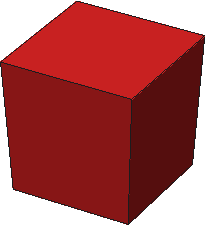
\includegraphics[width=\textwidth]{cubo}%
       	\label{subfig:cubo}%
    \end{subfigure}%
    %
    \hspace{1.5cm}
    %
    \begin{subfigure}[b]{0.2\textwidth}
       	\includegraphics[width=\textwidth]{prisma}%
       	\label{subfig:prisma}%
    \end{subfigure}%
    %
    \caption{Ejemplos de los objetos considerados para las clases $C_1$ (izquierda) y $C_2$ (derecha).}%
    \label{fig:objetos}%
\end{figure}
%
De los atributos posibles de estos objetos, el utilizado para diferenciar las clases de objetos es su altura $h$, el cual es suficiente para abordar el problema.

Así:
%
\begin{align}
	\label{eq:atributos_diferenciadores}
	A_k &= \{h_k\} \\
	\intertext{son los conjuntos de atributos asociados a cada objeto $o_k$, donde $h_k$ solo puede tener dos posibles valores, por lo cual las clases quedan definidas de la siguiente forma:}
	\begin{split}
		C_1  &= \{h_1\} \\[1em]
		C_2  &= \{h_2\} \rlap{${}= \{2h_1\}$}
	\end{split}
\end{align}
%
Para evaluar la propuesta en las diferentes configuraciones propuestas del espacio $E$, se utilizaron diferentes cantidades de objetos, siendo $N$ la cantidad total de objetos en dichos espacios, la cual será la suma de los objetos de ambas clases propuestas, donde $N_1$ es la cantidad de objetos de la clase $C_1$ y $N_2$ los objetos de la clase $C_2$. 

En los casos tratados solo se permite colocar un objeto por cada celda de la malla y la cantidad $N$ debe cumplir la desigualdad $\left\lceil \frac{nm}{2} \right\rceil < N \leq nm$.
Esto porque una cantidad de objetos igual o menor a $\left\lceil \frac{nm}{2} \right\rceil$ se considera un caso con solución trivial; ya que siempre se dispone de espacio suficiente para acomodarlos en una configuración en la cual se puedan tomar con una sola acción.
Además, el número de objetos disponibles no debe exceder el número total de celdas.
 
Dicho lo anterior, los casos de interés para validar la propuesta de este trabajo, consisten en todas las configuraciones de objetos $N_1$ y $N_2$ que no correspondan a casos triviales ni imposibles (los cuales serán detallados en la Sección \ref{sec:casos_triviales_e_imposibles}).
Es por ello que se obtuvieron las condiciones para que un caso no sea trivial ni imposible, resultando las siguientes:
%
\begin{equation}
\label{eq:cond_casos_de_interes}
\begin{gathered}
	\left\lceil \frac{nm}{2} \right\rceil < N \leq nm \\[7pt]
	N = N_1 + N_2 \\[7pt]
	0 \leq N_1 \leq N - \left\lfloor \frac{n}{2} \right\rfloor \! \left\lfloor \frac{m}{2} \right\rfloor \\[7pt]
	0 \leq N_2 \leq N - \left\lfloor \frac{n}{2} \right\rfloor \! \left\lfloor \frac{m}{2} \right\rfloor
\end{gathered}
\end{equation}
%
Un análisis más profundo de estas condiciones se dará en la Sección \ref{sec:casos_triviales_e_imposibles}.
%
%
\subsection{Características de la vecindad}
\label{subsec:vecindad}
%
%
Para definir el estado de la vecindad $V_{ij}$ de una celda $e_{ij}$, se considerarán como celdas vecinas de una celda particular $e_{ij}$, aquellas celdas que se encuentran inmediatamente arriba (dirección positiva de $i$), abajo, a la derecha (dirección positiva de $j$) y a la izquierda de esta, como se ilustra en la Figura \ref{fig:vecindad}.
%
\begin{figure}[H]
	\includegraphics[width=0.6\textwidth]{vecindad}%
	\caption{Vecindad utilizada para abordar el problema planteado.}%
	\label{fig:vecindad}%
\end{figure}
%
El orden en el que se encuentran los estados de las celdas vecinas en el conjunto $V_{ij}$ se obtiene recorriendo las posiciones mencionadas en sentido horario comenzando con la celda de arriba, es decir:
%
\begin{equation}
	\label{eq:vecindad_usada}
	V_{ij} = \{v_1, v_2, v_3, v_4\}
\end{equation}
%
donde:
%
\begin{descriptionParams}
	\item[$v_1$] corresponde al estado de la celda $e_{i+1,\, j}$.
	\item[$v_2$] corresponde al estado de la celda $e_{i,\, j+1}$.
	\item[$v_3$] corresponde al estado de la celda $e_{i-1,\, j}$.
	\item[$v_4$] corresponde al estado de la celda $e_{i,\, j-1}$.
\end{descriptionParams}
%
Las características de la vecindad de los elementos en los bordes y esquinas de la malla no difiere de las de los demás elementos.
Esto debido a que en todos los arreglos tratados se considera un ``espacio extendido'' de trabajo, el cual consiste en suponer que el espacio $E$ se encuentra rodeado por celdas vacías, tal y como se muestra en la Figura \ref{fig:malla_extendida}.
En estas celdas hipotéticas no se puede colocar ningún objeto, ya que únicamente cumplen con la función de actuar como vecinas de los elementos en los bordes y esquinas de la malla, de manera que las mismas reglas de vecindad de los elementos centrales también puedan ser aplicadas en ellos.
%
\begin{figure}[H]
	\includegraphics[width=0.6\textwidth]{malla_extendida_3D}%
	\caption{Ejemplo de espacio extendido en una malla de $4\times 4$.}%
	\label{fig:malla_extendida}%
\end{figure}
%
En todos los casos del presente trabajo se supondrá un espacio extendido como el de la Figura \ref{fig:malla_extendida}, pero esta característica puede ser modificada según las necesidades del problema que se aborde.
Por ejemplo, si se desea realizar el acomodo de objetos dentro de una caja, puede ser más adecuado cambiar las celdas vacías del espacio extendido por elementos fijos de determinada altura, a manera de pared.
%
%
\subsection{Formas de sujeción}
\label{subsec:formas_sujecion}
%
%
Solo se consideran dos formas de agarre, las cuales son comunes a ambas clases de objetos: agarre horizontal $H$ y agarre vertical $V$; esto es:
%
\begin{equation}
\label{eq:formas_sujecion_usadas}
	S = S_1 = S_2 = \{H, V\}
\end{equation}
%
Estas formas de agarre se establecieron considerando un manipulador que solo puede tomar los objetos por la parte superior. 
Un esquema de los puntos que son utilizados, en teoría, para sujetar los objetos se muestra en la Figura \ref{fig:formas_sujecion}.
%
\begin{figure}[H]
	\begin{subfigure}{0.4\textwidth}
		\includegraphics[width=\textwidth]{agarre_horizontal}%
		\label{subfig:sujecion_H}%
	\end{subfigure}%
	%
	\hspace{1cm}
	%
	\begin{subfigure}{0.4\textwidth}
		\includegraphics[width=\textwidth]{agarre_vertical}%
		\label{subfig:sujecion_V}%
	\end{subfigure}%
	\caption{Formas de sujeción horizontal (izquierda) y vertical (derecha).}%
	\label{fig:formas_sujecion}%
\end{figure}
%
%
\subsection{Restricciones de las formas de sujeción}
\label{subsec:restricciones}
%
%
Las formas de sujeción aplicables a cada clase de objeto pueden ser restringidas en función de su vecindad $V_{ij}$.
	
Un objeto $o_k$ puede ser sujetado de las formas $H$ y $V$ si sus vecinos horizontales y verticales, respectivamente, tienen una menor altura que el objeto $o_k$.
La definición matemática de la oración anterior se presenta en la Ecuación \ref{eq:restricciones} de la Sección \ref{sec:funciones_y_procedimientos}.

Algunos ejemplos de cómo se restringen las formas de sujeción de un objeto, en función de su vecindad se muestran en la Figura \ref{fig:restricciones_agarre}.
%
\begin{figure}[H]
	\def\hsep{12pt}%
	\captionsetup[subfigure]{width=\textwidth}%
	\begin{subfigure}{0.31\textwidth}
		\includegraphics[width=\textwidth]{restriccion_H_cubo}%
		\label{subfig:restriccion_H_cubo}%
	\end{subfigure}%
	\hspace{\hsep}%
	\begin{subfigure}{0.31\textwidth}
		\includegraphics[width=\textwidth]{restriccion_V_cubo}%
		\label{subfig:restriccion_V_cubo}%
	\end{subfigure}%
	\hspace{\hsep}%
	\begin{subfigure}{0.31\textwidth}
		\includegraphics[width=\textwidth]{restriccion_HV_cubo}%
		\label{subfig:restriccion_HV_cubo}%
	\end{subfigure}%
	
	\vspace{0.7cm}
	%
	\begin{subfigure}{0.31\textwidth} 
		\includegraphics[width=\textwidth]{restriccion_H_prisma}%
		\label{subfig:restriccion_H_prisma}
	\end{subfigure}%
	\hspace{\hsep}%
	\begin{subfigure}{0.31\textwidth}
		\includegraphics[width=\textwidth]{restriccion_V_prisma}%
		\label{subfig:restriccion_V_prisma}
	\end{subfigure}%
	\hspace{\hsep}%
	\begin{subfigure}{0.31\textwidth}
		\includegraphics[width=\textwidth]{restriccion_HV_prisma}%
		\label{subfig:restriccion_HV_prisma}%
	\end{subfigure}%
	%
	\caption{Ejemplos de cómo se pueden restringir las formas de sujeción en función de la vecindad.}%
	\label{fig:restricciones_agarre}%
\end{figure}
%
%
\subsection{Acciones}
\label{subsec:acciones}
%
%	
Por el momento solo se consideran dos tipos de acciones: poner un objeto en $E$ ($w_1$) y quitarlo de $E$ ($w_2$), es decir:
%
\begin{equation}
	\label{eq:acciones_usadas}
	W = \{w_1, w_2\}
\end{equation}
%
Se considera que estas acciones son suficientes para la primera aproximación propuesta para el problema planteado. 
%
%
\subsection{Especificaciones adicionales}
\label{subsec:especificaciones_adicionales}
%
%	
Los objetos no se pueden colocar uno encima de otro, por lo cual solo se pueden generar acomodos como el que se muestra en la Figura \ref{fig:muestra_acomodo}.
	
A diferencia del problema del contenedor, no se toma en cuenta el caso en que haya que dejar objetos sin acomodar por falta de espacio.
Ya que, si bien este sería un caso de estudio interesante, en el que se podrían fusionar las técnicas del problema del contenedor con las propuestas, se cree que el añadir este tipo de restricciones disfrazaría la esencia del verdadero problema que se quiere resolver.
Por lo cual se da por hecho que los $N$ objetos se pueden colocar sin problemas en $E$, es decir, ningún objeto debe quedar fuera de $E$ en el arreglo final.
%
\begin{figure}[H]
	\includegraphics[width=0.63\textwidth]{arreglo_muestra}%
	\caption{Ejemplo de una configuración de objetos en la malla.}%
	\label{fig:muestra_acomodo}%
\end{figure}
%
%
\section{Análisis de complejidad del problema}
\label{sec:analisis_complejidad}
%
%
Debido a que el objetivo final del presente trabajo es encontrar una configuración específica de los objetos de $O$ en $E$, la complejidad del problema estará entonces relacionada con el total de configuraciones de objetos que se pueden generar a partir de dados: un conjunto $O$ de objetos y un espacio $E$ en el cual colocarlos.  

Si se considera el espacio de búsqueda sobre todas las configuraciones posibles de objetos en la malla, utilizando el conjunto $O$ para la representación de los objetos y el símbolo $\boxslash$ para la representación de una celda vacía, se tiene el siguiente espacio de búsqueda:
%
\begin{equation}
	\label{eq:complejidad_1}
	\mathcal{C} = (O \cup \{ \boxslash \})^{nm}
\end{equation}
%
donde se ha hecho explícita la unión con la representación de una celda vacía, al considerarla como un elemento más del conjunto, debido a su recurrente uso.

Al utilizar el conjunto $O$ para la representación de los objetos, implícitamente se está considerando a cada uno de sus elementos como diferente a los demás, ya que, en general, sus respectivos atributos $A_k$ pueden ser diferentes.
Por lo cual el número de configuraciones posibles en dicho espacio viene dado por: 
%
\begin{equation}
	\label{eq:complejidad_2}
	|\mathcal{C}| = |O \cup \{ \boxslash \}|^{nm} = (N+1)^{nm}
\end{equation} 
%
Con la finalidad de reducir este espacio de búsqueda es que se ha establecido el sistema de clases definido anteriormente.
Mediante esta herramienta es posible identificar atributos clave $A_k$ de objetos no necesariamente iguales, los cuales permitan tratarlos como tal únicamente en lo que respecta a su sujeción.
Por ejemplo, si al tener una esfera y un cubo en el espacio $E$ se tiene la condición de que el manipulador solo es capaz de tomar estos objetos mediante una única posición y orientación, utilizando puntos de contacto semejantes; entonces, no tendría caso considerar estos objetos como diferentes, en lo que a su manipulación se refiere.
Por lo cual, para cuestiones de sujeción, lo conveniente sería representarlos como objetos de la misma clase.

Al hacer esta consideración el espacio de búsqueda puede ser reducido, ya que:
%
\begin{equation}
	\label{eq:complejidad_3}
	|C| \leq |O|
\end{equation}
%
por lo cual el nuevo espacio de búsqueda sería:
%
\begin{equation}
	\label{eq:complejidad_4}
	\mathcal{C}' = (C \cup \{ \boxslash \})^{nm}
\end{equation}
%
Y de forma similar a la Ecuación \ref{eq:complejidad_2}, el número de configuraciones posibles quedaría como:
%
\begin{equation}
	\label{eq:complejidad_5}
	|\mathcal{C}'| = |C \cup \{ \boxslash \}|^{nm} = (N_C+1)^{nm}
\end{equation}
%
Sin embargo, el espacio de búsqueda de interés para el problema enunciado, es un subconjunto de $\mathcal{C}'$, para el cual se tiene un número de objetos $N$ fijo, e igualmente las cantidades de objetos de cada clase $N_1, N_2, \ldots, N_{N_C}$ son también fijas.

Entonces, se define $\mathcal{C}''$ como el espacio de todas las configuraciones posibles de $N$ objetos de $N_C$ clases en un $E$ específico, donde $N_1, N_2, \ldots, N_{N_C}$ son cantidades fijas.
Para lo cual se define a $\mathcal{C}''_{\text{ins}}$ como cualquier instancia de $\mathcal{C}''$ y a $\mathcal{C}''_{\text{ins}}(C_K)$ como el número de veces que aparece la clase $C_K$ en $\mathcal{C}''_{\text{ins}}$.
Por lo tanto 
%
\begin{equation}
	\label{eq:complejidad_6}
	\mathcal{C}'' = (C \cup \{ \boxslash \})^{nm} \ | \ \mathcal{C}''_{\text{ins}}(C_K) = N_K,\ 1 \leq K \leq N_C
\end{equation}
%
lo cual establece que debe haber exactamente $N_1$ objetos de la clase $C_1$, $N_2$ de la clase $C_2$, etc., en cualquier instancia de $\mathcal{C}''$.

El número de configuraciones posibles para $\mathcal{C}''$ es entonces:
%
\begin{equation}
	\label{eq:complejidad_7}
	|\mathcal{C}''| = \frac{nm!}{N_1!N_2! \cdots N_{N_C}!(nm - N)!}
\end{equation}
%
En la Tabla \ref{tab:permutaciones_posibles} se muestra el número de configuraciones posibles para algunas combinaciones de valores del tamaño de la malla y del número de objetos de cada clase.
%
\begin{table}[H]
	\renewcommand{\arraystretch}{1.4}%
	\savetablewidth{%
	\begin{tabular}{ccccc}
		\hline
		\textbf{Tamaño malla} & $\bm{N_1}$ & $\bm{N_2}$ & $\bm{nm-N}$ & $\bm{|\mathcal{C}''|}$ \\ \hline
		\arrayrulecolor{gray!60}%
		$3\times 3$ & $3$ & $3$ & $3$ & $\num{1680}$ \\ \hline
		$3\times 3$ & $1$ & $5$ & $3$ & $504$ \\ \hline
		$3\times 3$ & $4$ & $5$ & $0$ & $126$ \\ \hline
		$4\times 4$ & $5$ & $5$ & $6$ & $\num{2018016}$ \\ \hline
		$4\times 4$ & $1$ & $9$ & $6$ & $\num{80080}$ \\ \hline
		$4\times 4$ & $8$ & $8$ & $0$ & $\num{12870}$ \\ \hline
		$5\times 5$ & $8$ & $8$ & $9$ & $2.62\times10^{10}$ \\ \hline
		$5\times 5$ & $10$ & $10$ & $5$ & $0.98\times10^{10}$ \\ \hline
		$5\times 5$ & $12$ & $13$ & $0$ & $\num{5200300}$ \\ \hline
		$6\times 6$ & $12$ & $12$ & $12$ & $3.38\times10^{15}$ \\ \hline
		$6\times 6$ & $15$ & $15$ & $6$ & $0.30\times10^{15}$ \\ \hline
		$6\times 6$ & $18$ & $18$ & $0$ & $9.07\times10^{9}$ \\ 
		\arrayrulecolor{maintextcolor}%
		\hline
	\end{tabular}%
	}%
	\captionsetup{width=\tablewidth}%
	\caption{Número de permutaciones de arreglos posibles en función del número de elementos de cada clase presentes en la malla y del tamaño de la malla.}%
	\label{tab:permutaciones_posibles}%
\end{table}
%
Al analizar la Tabla \ref{tab:permutaciones_posibles} se puede observar que, entre más uniforme sea la distribución del número de objetos de cada clase y de celdas vacías ($nm - N$), el número de permutaciones posibles de una malla aumenta.
Es decir, que cuando las cantidades de objetos de cada clase y de celdas vacías son lo más parecidas entre sí, es cuando el número de permutaciones es máximo, y disminuye conforme se va perdiendo esta uniformidad.
%
%
\section{Casos triviales y casos imposibles}
\label{sec:casos_triviales_e_imposibles}
%
%
Existen cantidades especiales de objetos $N$, así como del número de objetos de cada clase $N_1, N_2, \ldots, N_{N_C}$, para las cuales se pueden tener casos de acomodo triviales o imposibles.
Las características de estos casos se definen a continuación.

Un caso trivial es un caso en el cual la cantidad $N$ de objetos es lo suficientemente pequeña como para acomodar los objetos en un patrón simple, el cual permite que todos los objetos puedan ser sujetados con una sola acción.
En este caso los objetos pueden ser siempre colocados mediante un mismo patrón, previamente establecido, siempre que se cumpla la siguiente condición:
%
\begin{equation}
	\label{eq:condicion_triviales}
	N \leq \left\lceil \frac{nm}{2} \right\rceil
\end{equation}
%
Un patrón de acomodo para casos triviales se presenta en la Figura \ref{fig:casos_triviales}, dónde $N = \left\lceil \frac{nm}{2} \right\rceil$.
En el presente trabajo no se abordan este tipo de casos.
%
\begin{figure}[H]
    \begin{subfigure}{0.3\textwidth}
		\includegraphics[width=\textwidth]{arreglo_trivial_4x4_2D}%
       	\label{subfig:trivial_4x4}%
    \end{subfigure}%
    %
    \hspace{2.2cm}
    %
    \begin{subfigure}{0.3\textwidth}
       	\includegraphics[width=\textwidth]{arreglo_trivial_5x5_2D}%
       	\label{subfig:trivial_5x5}%
    \end{subfigure}%
    %
    \caption{Ejemplos de casos triviales en mallas de $4\times 4$ (izquierda) y $5\times 5$ (derecha).}
    \label{fig:casos_triviales}%
\end{figure}
%
Por otro lado, también existen configuraciones específicas de objetos en la malla, las cuales implican que algunos objetos sean imposibles de tomar, dadas las reglas de sujeción establecidas.
Estos casos se presentan cuando al menos cuatro objetos de la misma clase se agrupan en un patrón como el que se muestra en la subfigura izquierda de la Figura \ref{fig:casos_imposibles}.
En este caso ninguno de los cuatro objetos puede ser sujetado mediante las formas de sujeción definidas $H$ y $V$.
Estas agrupaciones de cuatro elementos de la misma clase se puede presentar una o varias veces en un acomodo de objetos, como se muestra en la subfigura derecha de la Figura \ref{fig:casos_imposibles}.

Se ha denominado como \textsl{cuadro imposible} al arreglo de cuatro objetos de la misma clase descrito anteriormente, y como \textsl{caso imposible} a un arreglo de objetos en la malla que contenga al menos un cuadro imposible.
%
\begin{figure}[H]
	\begin{subfigure}{0.3\textwidth}
		\includegraphics[width=\textwidth]{arreglo_imposible1_4x4_2D}%
   		\label{subfig:imposibles_1}%
	\end{subfigure}%
	%
	\hspace{2.2cm}
	%
	\begin{subfigure}{0.3\textwidth}
		\includegraphics[width=\textwidth]{arreglo_imposible2_4x4_2D}%
		\label{subfig:imposibles_2}%
	\end{subfigure}%
	%
	\caption{Ejemplos de casos imposibles.}%
	\label{fig:casos_imposibles}%
\end{figure}
%
Los casos imposibles como los de la Figura \ref{fig:casos_imposibles} se pueden evitar con un acomodo correcto de los objetos en la malla.
Sin embargo existe una condición, la cual implica que siempre habrá cuadros imposibles en la malla, sin importar la forma en que se acomoden los objetos.

La condición para que exista al menos un cuadro imposible en un arreglo de objetos es:
%
\begin{equation}
	\label{eq:condicion_imposibles}
	\max_{K} N_K > nm - \left\lfloor \frac{n}{2} \right\rfloor \! \left\lfloor \frac{m}{2} \right\rfloor
\end{equation}
%
En el presente trabajo no se abordan este tipo de casos.

En el siguiente capítulo se presentarán los procedimientos y algoritmos desarrollados para abordar el problema propuesto.
Al final del capítulo se presentará el algoritmo principal que resuelve el problema planteado, el cual hace uso de los procedimientos que le preceden.
Posteriormente, en el Capítulo \ref{chap:resultados}, se presentarán los resultados obtenidos al aplicar el algoritmo principal a diferentes tamaños de malla y diferentes combinaciones de cantidades de objetos en ellas.
Finalmente, en el Capítulo \ref{chap:conclusiones}, se abordarán las conclusiones del proyecto.